\section{Wakefields, Impedances and Beam Dynamics Effects}

\section{Theoretical Background of Wakefields and Impedances}

%
% Explaination of the concept of wakefields (the source and witness particle), oscillating electric fields
% induced by a charged particle. Longitudinal and Transverse wakefields

\begin{itemize}
\item{Wakes}
\begin{itemize}
\item{Introduction to the electromagnetic field of charged particle moving in free space}
\item{Field of a particle in a perfectly conducting pipe - method of image currents}
\item{Place a witness particle distance s behind source particle and deduce electric field as seen by this particle}
\item{normalise this by the source particle charge to give the wakepotential}
\item{And again by the source particle charge and current profile to acquire the loss factor}
\item{Longitudinal field predominantly}
\item{Introduce the Panowsky-Wenzel theorem covering transverse field - Transverse wakes}
\end{itemize}
\item{Impedance}
\begin{itemize}
\item{Firstly mention the commonality of frequency dependent material properties - ferrite permeability, permitivitty determined by conductivity/frequency in conductors/dielectrics/skin depth}
\item{Fourier transform of wakefield into the convolution of the beam current spectrum and the impedance}
\item{Again Panowsky-Wenzel for impedance}
\item{Discussion of the transverse impedance - in particular the general definition of an impedance (n-th order current interacting with an m-th order field)}
\item{Define dipolar/driving and quadrupolar/detuning impedance. In addition constant transverse impedance term}
\end{itemize}
\end{itemize}


\subsection{Resistive Wall Impedance}

\begin{itemize}
\item{Return to simple axisymmetric geometry concerning a finite conductivity of the wall}
\item{Derive in frequency domain - then have impedance. Give an example wakefield of a good conductor (copper), bad conductor (graphite), non-conductor (ferrite)}
\end{itemize}

\subsection{Geometric Impedance}
\begin{itemize}
\item{Derive the field pattern for a pillbox cavity - Oscillating fields with a characteristic frequency of some multiple of the lowest eigenfrequency}
\end{itemize}
\section{Examples of Effects}

\subsection{Beam Induced Heating}

\subsection{Defining and Deriving Power Loss in Circular Accelerators}
\label{sec:power_loss}

When a charged particle interacts with an impedance it losses energy to generate the resulting wakefield. This is called the parasitic loss, and is generally defined as[ref Chao/Ng]

\begin{equation}
\Delta E = -2\pi e^{2}N_{b}\int^{\infty}_{-\infty} d\omega \left| \lambda \left( \omega \right)  \right|^{2} Z_{\parallel} \left( \omega \right)
\end{equation}

where $\Delta E$ is the energy loss per pass per particle, $e$ is the charge per particle, $N_{b}$, $\omega$ the frequency, $\lambda$ the line density of the bunch and $Z_{\parallel}$ the longitudinal impedance of the object being traversed.
																
Due to the decay of the wakefields induced by this energy loss, this energy must eventually be lost to the device causing the impedance (valid below the cutoff frequency of the machine beam pipe). Therefore we can assume that the energy loss from the particles is absorbed by the surrounding structure. Summing over all particles in a bunch we can therefore obtain a sum of the energy loss;

\begin{equation}
\Delta E_{bunch} = 2\pi \left( eN_{b}   \right)^{2} \int^{\infty}_{-\infty} d\omega \left| \lambda \left( \omega \right)  \right|^{2} Z_{\parallel} \left( \omega \right)
\end{equation}

As often we must deal with machines storing multiple bunches, for these we simply multiply the energy loss per bunch by the number of stored bunches to acquire the total energy loss per passage;

\begin{equation}
\Delta E_{bunches} = 2\pi \left( eN_{b}   \right)^{2}n_{bunch}\rho \int^{\infty}_{-\infty} d\omega \left| \lambda \left( \omega \right)  \right|^{2} Z_{\parallel} \left( \omega \right)
\end{equation}

where $n_{bunch}$ is the number of bunches in the machine assuming all bunches being equally spaced, and $\rho$ is the fraction of the machine occupied in operation. If we assume a revolution frequency $f_{rev}$ we thus get a power loss of;

\begin{align}
P_{loss}  = & \Delta E_{bunches} f_{rev}\nonumber \\  
 = & 2\pi f_{rev} \left( eN_{b}   \right)^{2}n_{bunch}\rho \int^{\infty}_{-\infty} d\omega \left| \lambda \left( \omega \right)  \right|^{2} Z_{\parallel} \left( \omega \right) \nonumber  \\ 
 = & 2\pi f_{rev} \left( eN_{b}   \right)^{2}n_{bunch}\rho \int^{\infty}_{-\infty} d\omega \left| \lambda \left( \omega \right)  \right|^{2} Z_{\parallel} \left( \omega \right) \nonumber \\
 = & 2\pi f_{rev} \left( eN_{b}   \right)^{2}n_{bunch}\rho \int^{\infty}_{-\infty} d\omega \left| \lambda \left( \omega \right)  \right|^{2} \left( \Re{}e \left( Z_{\parallel} \left( \omega\right) + \Im{}m Z_{\parallel} \left( \omega\right) \right) \right).
\end{align}
 
As $\Re{}e\left(Z_{\parallel} \left( \omega\right)\right)$ is an even function and $\Im{}m\left(Z_{\parallel} \left( \omega\right)\right)$ is an odd function, we see that

\begin{equation}
P_{loss}   =  \omega_{rev} \left( eN_{b}   \right)^{2}n_{bunch}\rho \int^{\infty}_{0} 2 d\omega \left| \lambda \left( \omega \right)  \right| ^{2}  \Re{}e \left( Z_{\parallel} \left( \omega\right)  \right).
\end{equation}

Next we make a change of the variable of integration $\omega = n_{bunch}\omega_{rev}$;

\begin{equation}
P_{loss}   =  \omega_{rev} \left( eN_{b}   \right)^{2}n_{bunch}^{2} \int^{\infty}_{0} 2 d\omega_{rev} \left| \lambda \left( \omega_{rev}n_{bunch} \right)  \right|^{2}  \Re{}e \left( Z_{\parallel} \left( \omega_{rev}n_{bunch}\right)  \right).
\end{equation}

We can subsequently change to a sum formalism to obtain

\begin{equation}
P_{loss} = \left( \omega_{rev}eN_{b}n_{bunch}  \right)^{2} \displaystyle\sum\limits_{p = 0}^{\infty} \left( 2 \left| \lambda \left(p \omega_{rev}n_{bunch} \right)  \right|^{2}  \Re{}e \left( Z_{\parallel} \left(p \omega_{rev}n_{bunch}\right) \right) \right) \label{ean:heating-gen}
\end{equation}

where $\omega_{0} = 2\pi f_{0}$, $f_{0} = \frac{1}{\tau_{b}}$ and $\tau_{b}$ is the bunch spacing.

\subsection{Longitudinal Beam Profiles}

As shown by the derivations in Section~\ref{sec:power_loss}, asides from the longitudinal impedance of the device under consideration the longitudinal profile of the circulating bunches also contributes to the power loss in the machine. In past works it has generally been assumed that bunches in accelerators have a Gaussian profile [ref Sacherer/Grudiev/Laclare](seen in Eqn.~\ref{eqn:gauss}, where $4\sigma_{z} = t_{b}$, $t_{b}$ is the bunch length) when approaching the analytical treatment of beam instabilities, both single-bunch and multi-bunch. Recent measurements of the power spectrum of particle beams, especially in the LHC [ref theo/phillipe] have shown characteristics that the Gaussian profile does not predict, for example the high frequency secondary peak as seen in Fig.~\ref{fig:measured_gauss}. To make more realistic predictions of heat loss due to beam impedance in the machine it is thus necessary to find bunch profiles which reproduce this behaviour.

\begin{equation}
\lambda \left( t \right) = e^{\frac{-t^{2}}{2\sigma^{2}}}
\label{eqn:gauss}
\end{equation}

\begin{figure}
\subfigure[]{
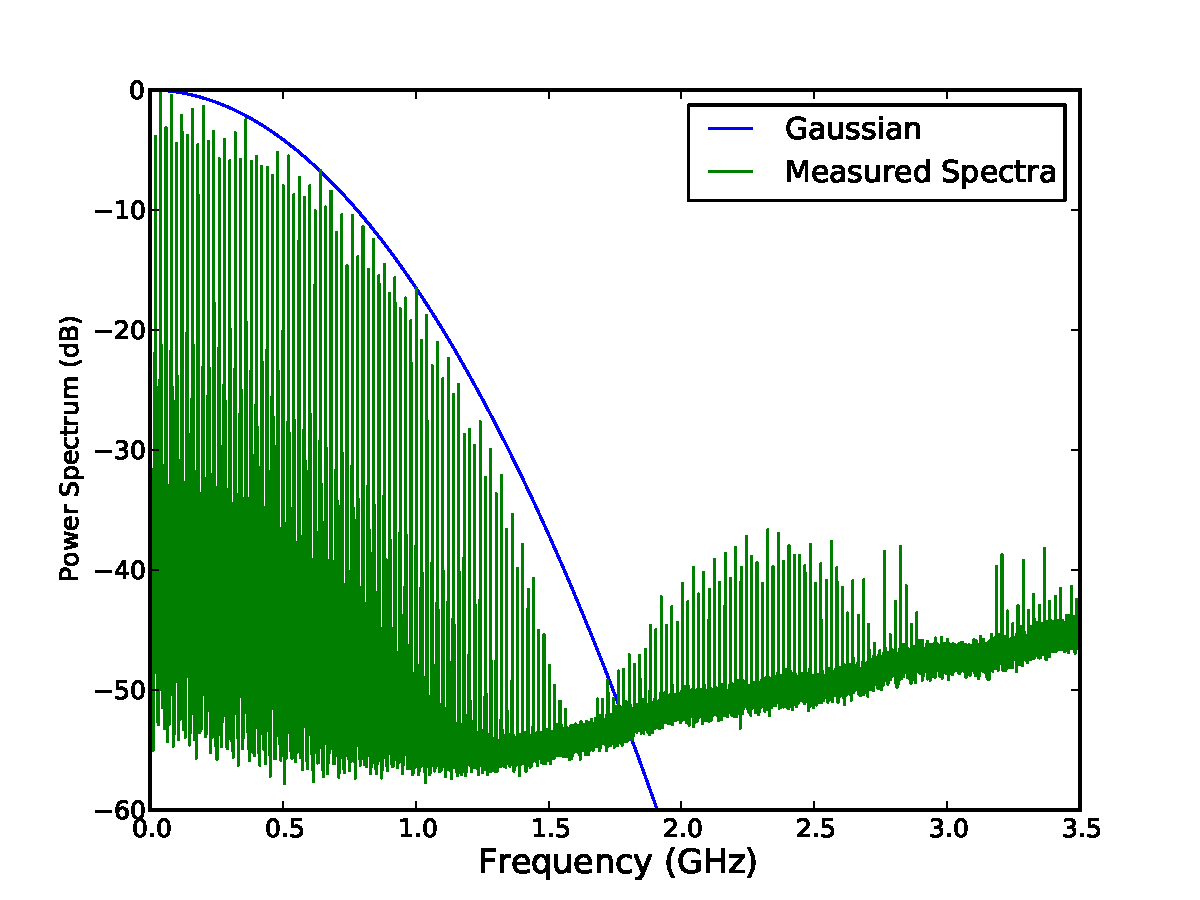
\includegraphics[width=0.45\textwidth]{figures/wakefields_and_impedance/beam_spectra_power_gauss_meas_12ns.pdf}
\label{fig:gauss_meas_freq}
}
\subfigure[]{
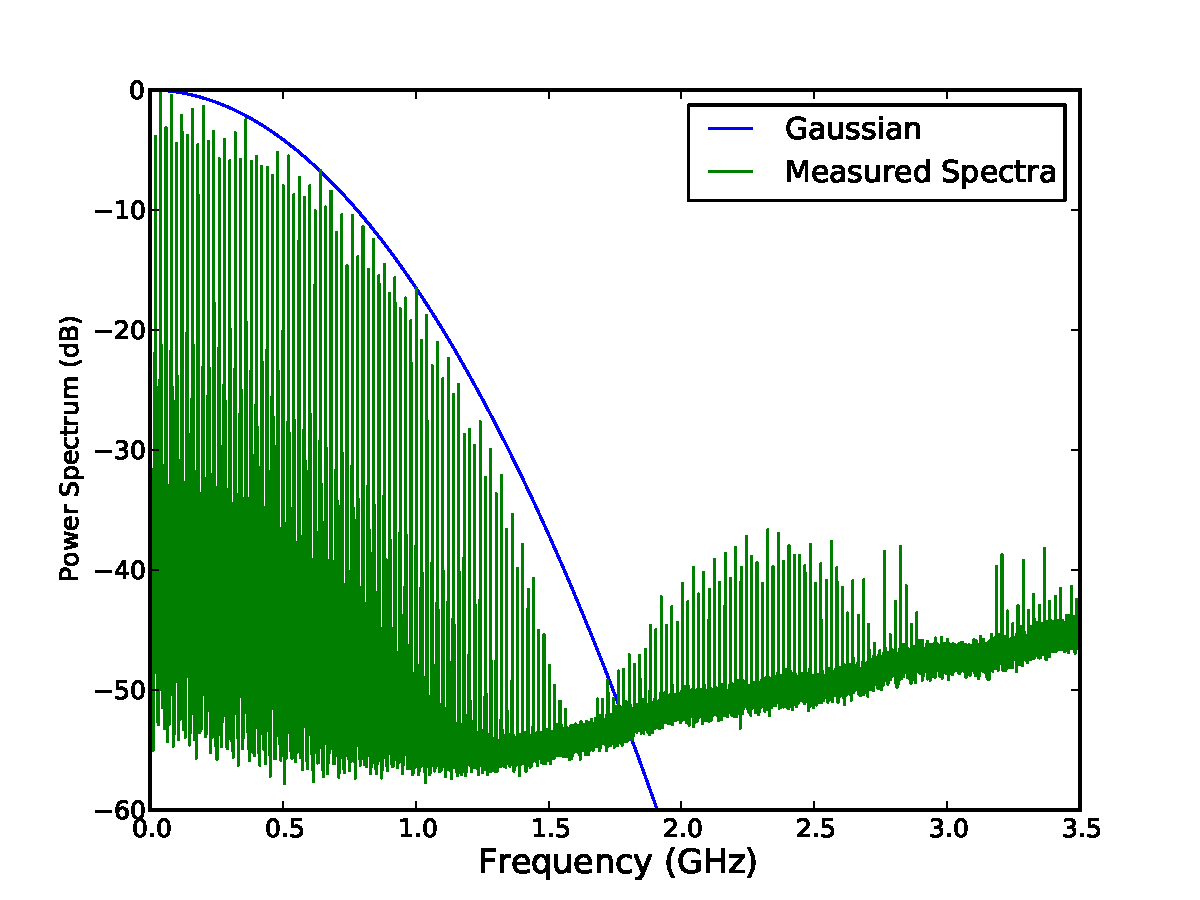
\includegraphics[width=0.45\textwidth]{figures/wakefields_and_impedance/beam_spectra_power_gauss_meas_12ns.pdf}
\label{fig:gauss_meas_time}
}
\caption{A comparison of \ref{fig:gauss_meas_freq} a measured beam power spectrum and a gaussian bunch of the same bunch length in the frequency domain and \ref{fig:gauss_meas_time} the resulting time domain beam profile. The gaussian has a bunch length (4$\sigma_{z}$ = 1.2ns) }
\label{fig:measured_gauss}
\end{figure}

A number of different longitudinal bunch profiles have been investigated in the past. Here we shall look at 3 other bunch profiles; a parabolic line density (see Eqn.~\ref{eqn:para_profile}), cos$^{2}$ (see Eqn.~\ref{eqn:cos_profile}), water-bag (see Eqn.~\ref{eqn:water_bag_profile}).

\begin{equation}
A\left( t \right) = \int^{\infty}_{-\infty} \lambda \left( \omega \right) e^{j\omega t} d\omega = 
\begin{cases}1-\left( \frac{2t} {t_{b}} \right)^{2} &\textrm{if $| t/2 | \leq t_{b}$}\\
0								&\textrm{if $| t/2 | > t_{b}$}
\end{cases}
\label{eqn:para_profile}
\end{equation}

\begin{equation}
A\left( t \right) = \int^{\infty}_{-\infty} \lambda \left( \omega \right) e^{j\omega t} d\omega = 
\begin{cases}
cos^{2}\left( \frac{\pi t} {t_{b}} \right) &\textrm{if $| t/2 | \leq t_{b}$}\\
0								&\textrm{if $| t/2 | > t_{b}$}
\end{cases}
\label{eqn:cos_profile}
\end{equation}

\begin{equation}
A\left( t \right) = \int^{\infty}_{-\infty} \lambda \left( \omega \right) e^{j\omega t} d\omega = 
\begin{cases}
\sqrt{1-\left( \frac{2t}{t_{b}}\right)^{2}} &\textrm{if $| t/2 | \leq t_{b}$}\\
0								&\textrm{if $| t/2 | > t_{b}$}
\end{cases}
\label{eqn:water_bag_profile}
\end{equation}

The comparison of these bunch profiles in the time domain are shown in Fig.~\ref{fig:time_bunch_profiles}. Note all bunch currents are normalised to their peak value. The corresponding current and power spectrums are shown in Fig.~\ref{fig:freq_dom_prof}. There are several things to note about these spectra; firstly that the non-infinite distribution of the non-gaussian bunch profiles gives rise to a number of high frequency lobes in the power spectrum, and secondly the interval of these nodes depends heavily on the bunch profile.

\begin{figure}
\begin{center}
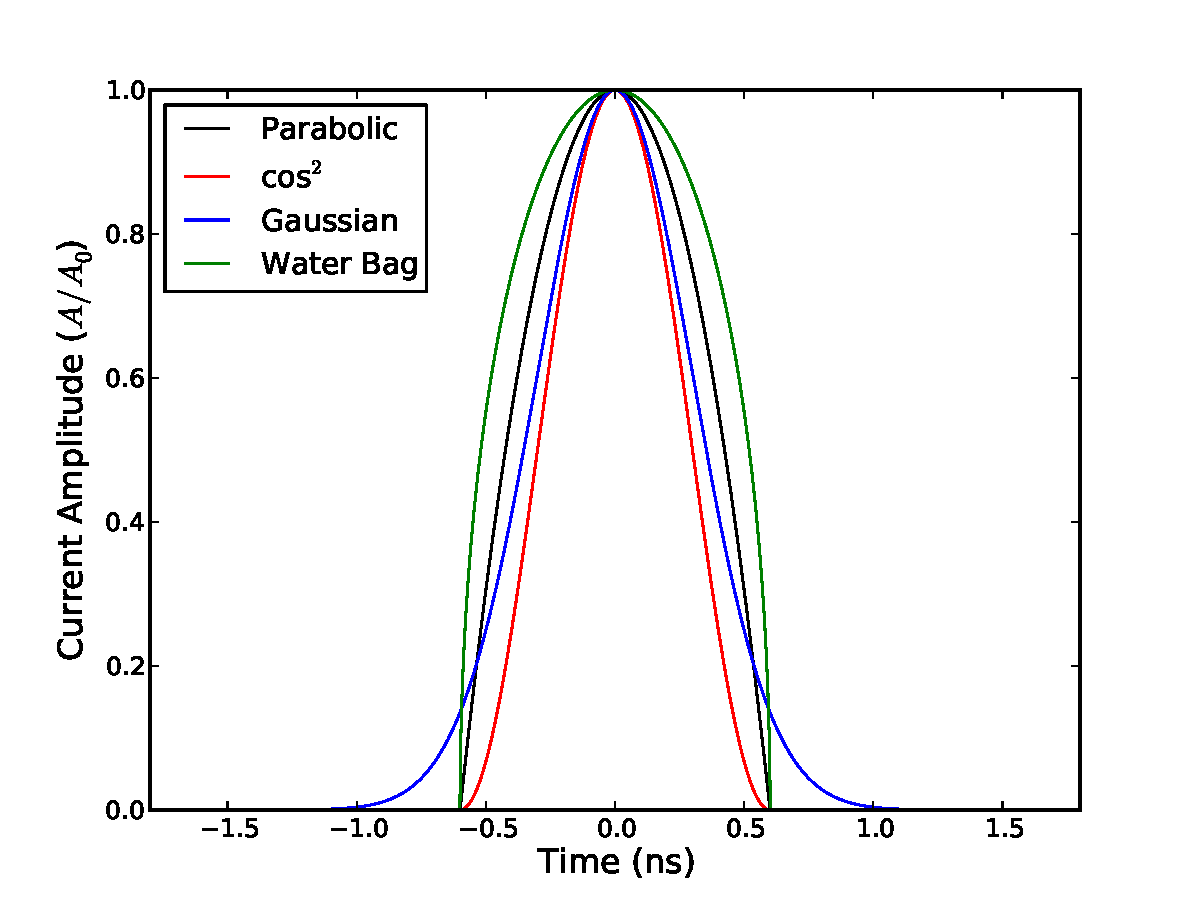
\includegraphics[width=0.65\textwidth]{figures/wakefields_and_impedance/bunch_profile_12ns.pdf}
\end{center}
\label{fig:time_bunch_profiles}
\caption{The longitudinal bunch profile of a number of bunch distributions. Note that all of them are normalised to have a peak bunch current of 1. For the gaussian distribution the bunch length is the 4$\sigma$ value. The bunch length $\tau_{b} = 1.2ns$}
\end{figure}

\begin{figure}
\subfigure[]{
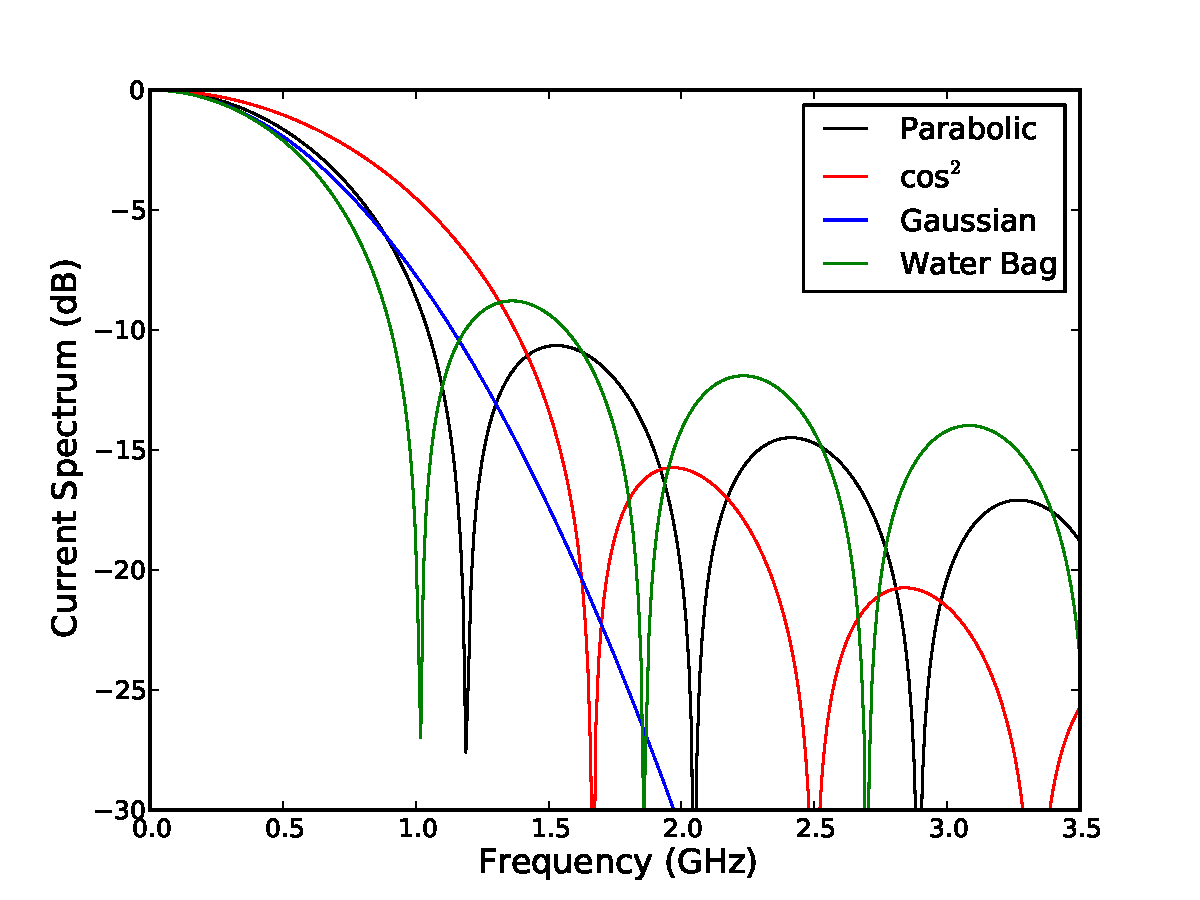
\includegraphics[width=0.45\textwidth]{figures/wakefields_and_impedance/current_spectrum_12ns.pdf}
\label{fig:current_spec}
}
\subfigure[]{
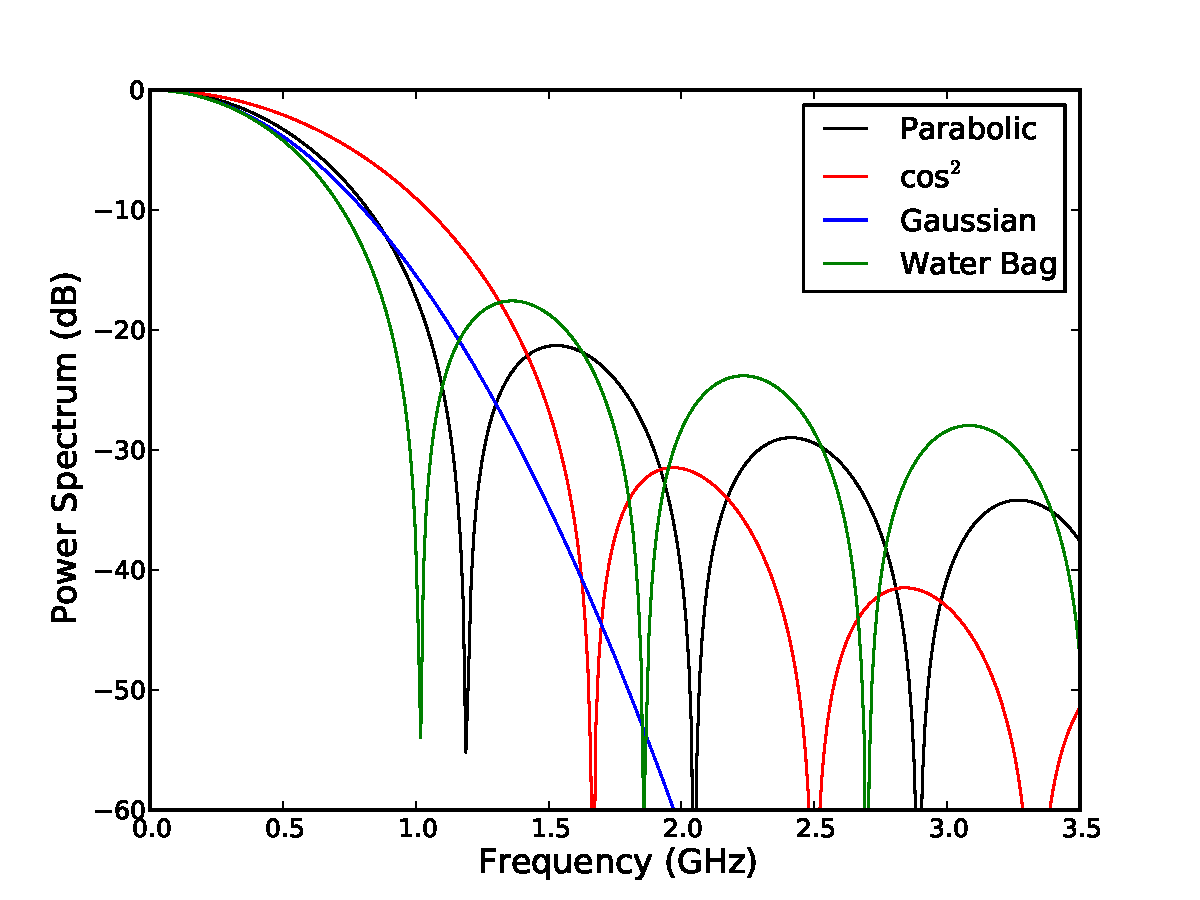
\includegraphics[width=0.45\textwidth]{figures/wakefields_and_impedance/power_spectrum_12ns.pdf}
\label{fig:power_spec}
}
\label{fig:freq_dom_prof}
\caption{The frequency domain \ref{fig:current_spec} current spectrum and \ref{fig:power_spec} power spectrum for a number of different bunch profiles with a bunch length $\tau_{b} = 1.2ns$.}
\end{figure}

To illustrate more clearly the effect of changing the bunch length on the power spectrum, a number of bunch profiles and the corresponding power spectra with different bunch lengths are shown below. Firstly, consider a gaussian bunch profile. It can be seen in Fig.~\ref{fig:diff_bunch_len_gauss} that by increasing the bunch length that the magnitude at high frequencies is decreased quite substantially as the bunch length increases. If we consider a finite bunch profile (non-gaussian), we note that we have high frequency lobes. The peak frequency of these lobes depends on the bunch length, as illustrated using a parabolic bunch profile for bunch lengths $\tau_{b} = 1ns, 1.2ns, 1.4ns$ in Fig.~\ref{fig:diff_bunch_len_para}. As the bunch length is increased the lobes move to lower frequencies, and the width of the first branch decreases, as seen for the gaussian bunch. Similar behaviour is observed with the cos$^{2}$ and water-bag bunch profiles.

\begin{figure}
\subfigure[]{
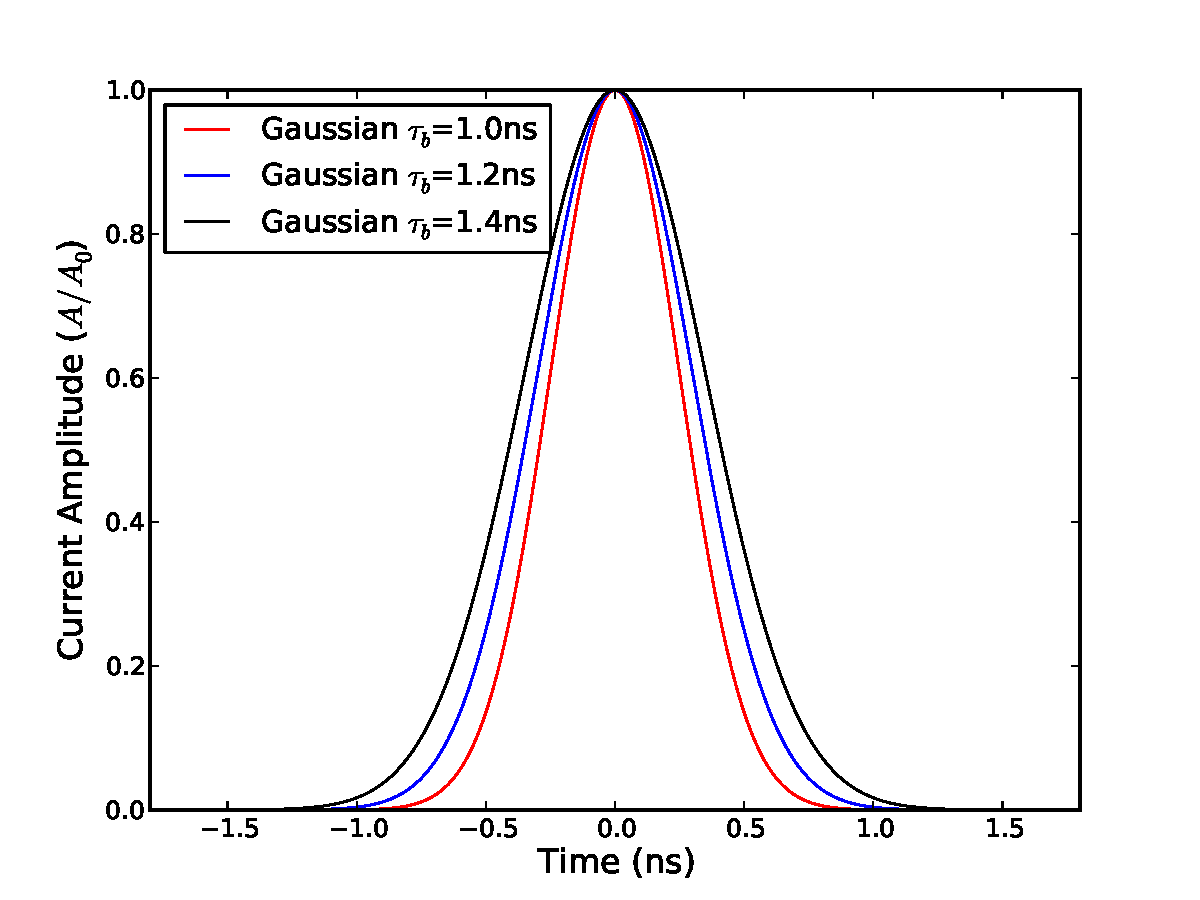
\includegraphics[width=0.45\textwidth]{figures/wakefields_and_impedance/gaussian_time_dom_diff_lengths.pdf}
\label{fig:change_len_time_gauss}
}
\subfigure[]{
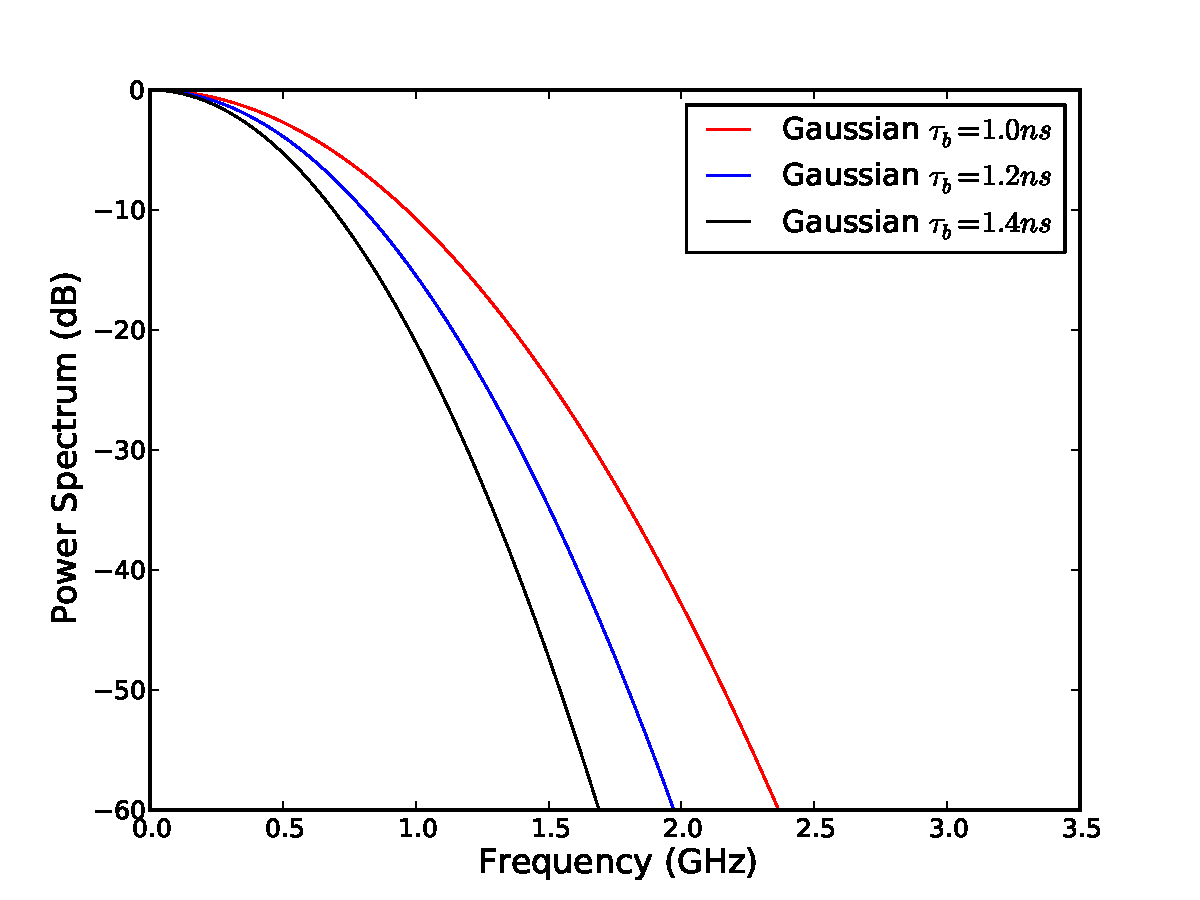
\includegraphics[width=0.45\textwidth]{figures/wakefields_and_impedance/gaussian_power_spec_diff_lengths.pdf}
\label{fig:change_len_freq_gauss}
}
\label{fig:diff_bunch_len_gauss}
\caption{\ref{fig:change_len_time_gauss} The longitudinal profile and the \ref{fig:change_len_freq_gauss} associated bunch power spectrum for a number of bunch lengths assuming a gaussian bunch profile.}
\end{figure}

\begin{figure}
\subfigure[]{
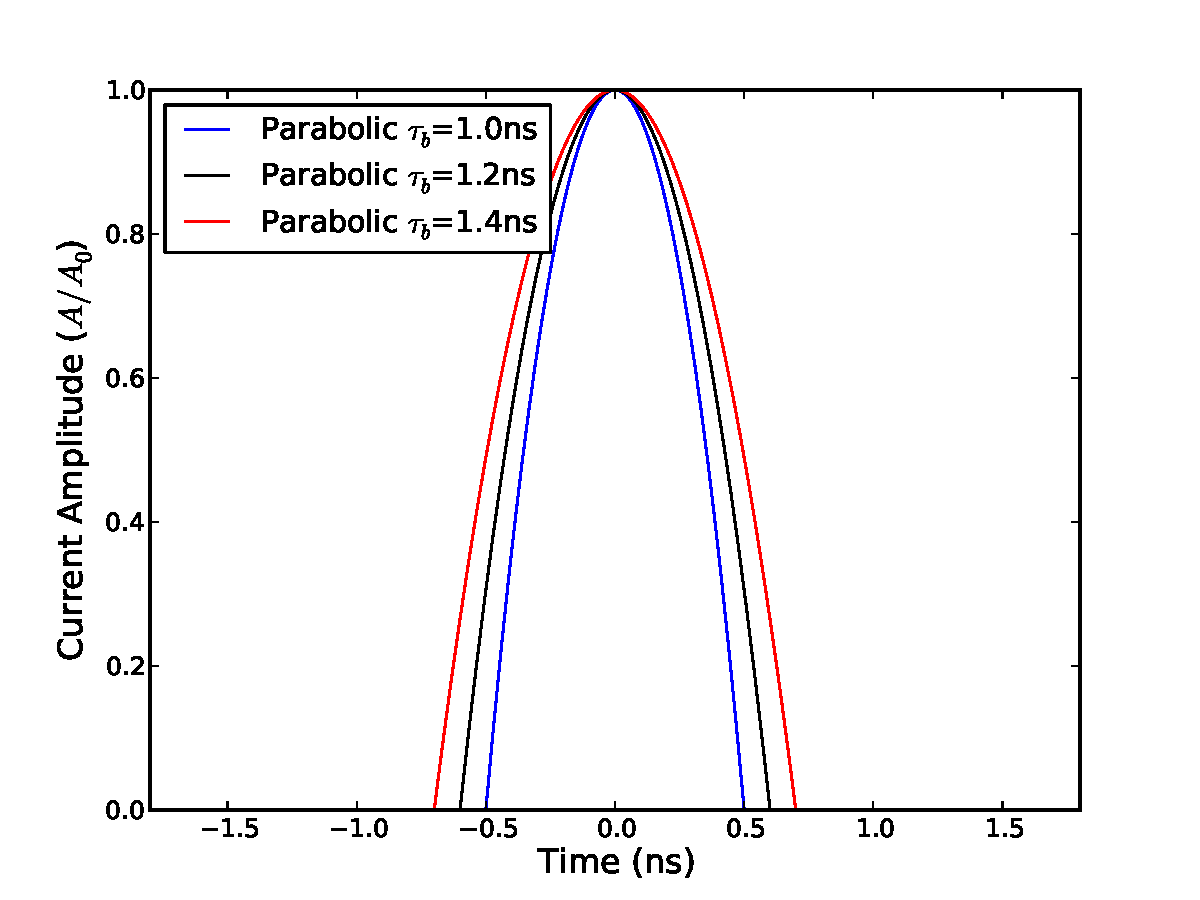
\includegraphics[width=0.45\textwidth]{figures/wakefields_and_impedance/current_amp_para_change.pdf}
\label{fig:change_len_time_para}
}
\subfigure[]{
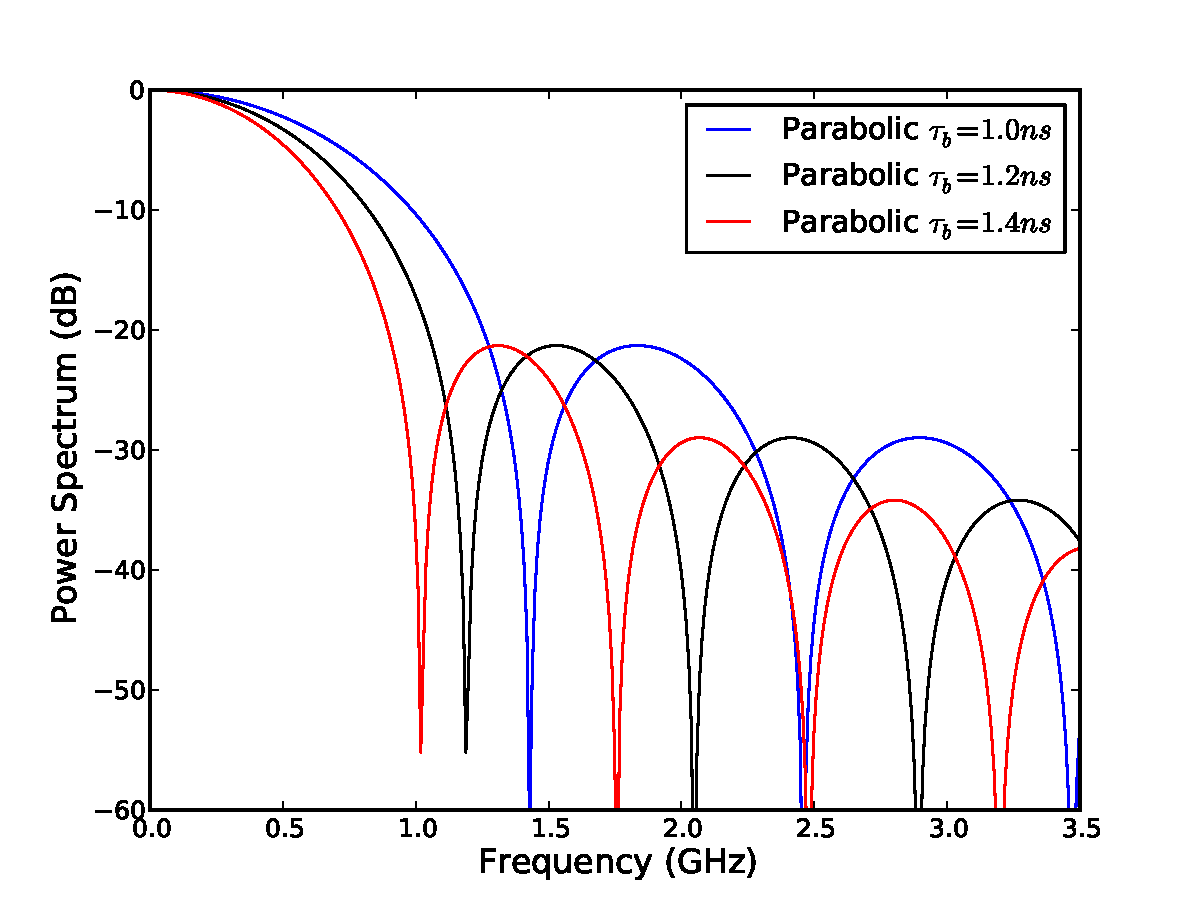
\includegraphics[width=0.45\textwidth]{figures/wakefields_and_impedance/freq_power_para_change.pdf}
\label{fig:change_len_freq_para}
}
\label{fig:diff_bunch_len_para}
\caption{\ref{fig:change_len_time_para} The longitudinal profile and the \ref{fig:change_len_freq_para} associated bunch power spectrum for a number of bunch lengths assuming a parabolic bunch profile.}
\end{figure}

Finally, a comparison of a measured bunch power spectra and the analytical power spectra is shown in Fig.~\ref{fig:power_all}. It can be seen that whilst it is possible to replicate some of the properties of the measured spectrum, an exact replication is non-trivial. Further investigation into the appropriate bunch profile is ongoing.

\begin{figure}
\begin{center}
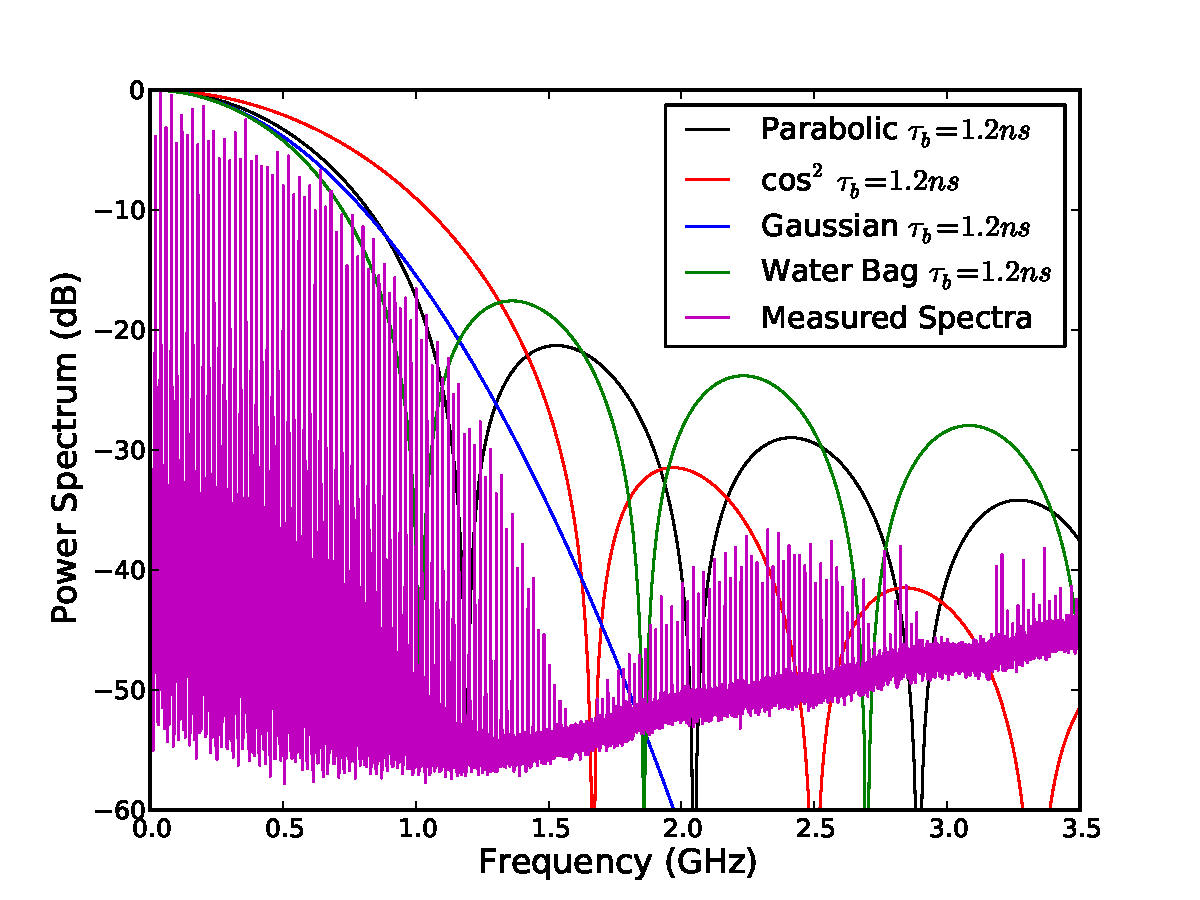
\includegraphics[width=0.65\textwidth]{figures/wakefields_and_impedance/beam_spectra_power_12ns.pdf}
\end{center}
\label{fig:power_all}
\caption{A comparison of a measured beam power spectrum and a number of analytical bunch profiles assuming a bunch length of 1.2ns.}
\end{figure}



% Introduce a number of longitudinal profiles in time domain - gaussian, parabolic line density, cos^2, water bag - comments of realism (gaussian being infinite) - truncated gaussian
% Comparison in the frequency domain - firstly gaussian compared to truncated gaussian - infinite tails reduce the magnitude of the higher frequency components and lobe
% Gaussian, parabolic, cos^2 - all with the same bunch length
% Using the above examples try using a number of different bunch lengths to illustrate how they change (gaussian - just extends further, parabolic, cos^2 lobe frequency changes)
% Finally - comparison to measured spectra to illustrate changes in bunch length and frequency components as bunch is ramped and squeezed

\subsection{Beam induced heating due to a low Q impedance}

%% Example done with a low Q (Q ~ 1/10)
%% To illustrate effect of bunch length increase
%% Illustrate change with number of bunches (linear)

For an impedance with a characteristic Q that is small (Q $<$ 10), it can be seen that the impedance peak will interact substantially with a number of beam harmonics (see Fig.~\ref{fig:low_q_harmonics}) due to the broad frequency range it occupies.

\begin{figure}
\begin{center}
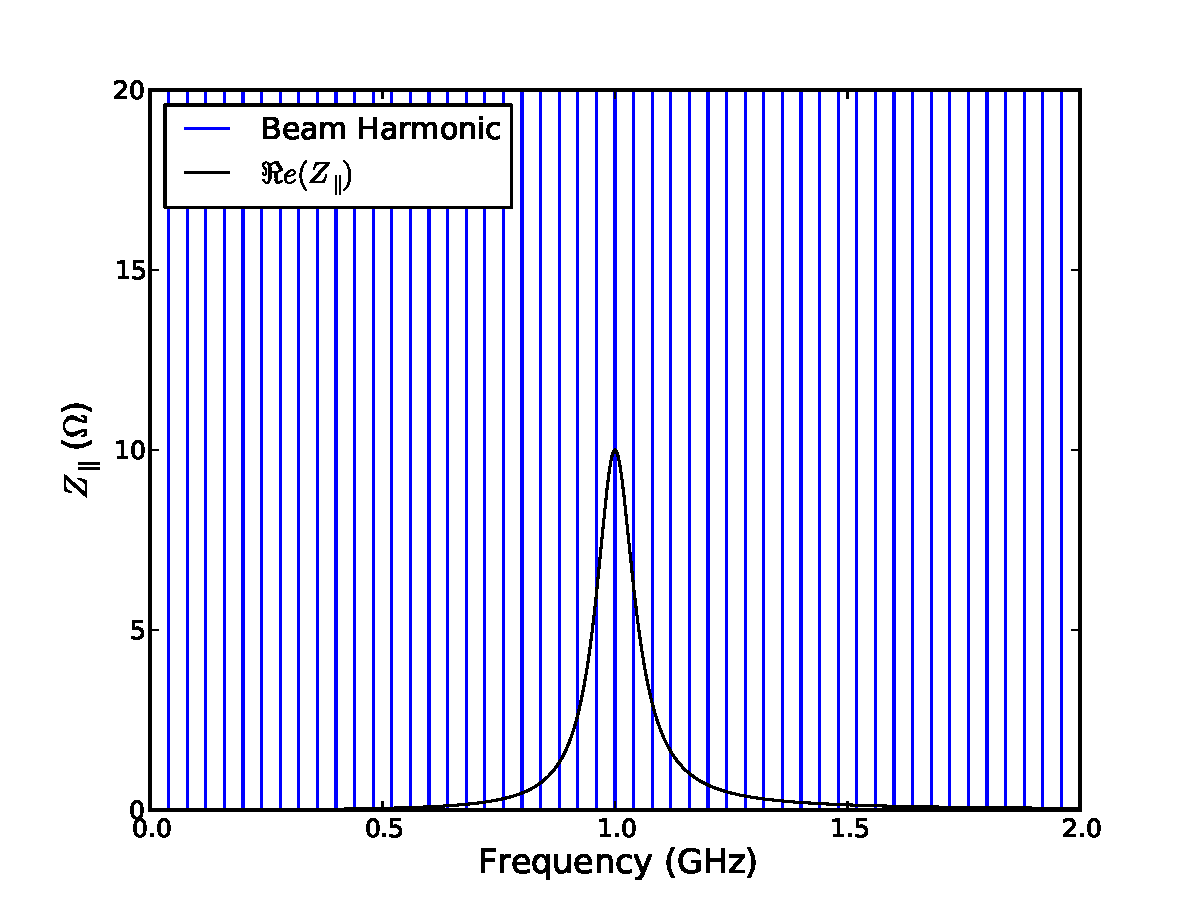
\includegraphics[width=0.65\textwidth]{figures/wakefields_and_impedance/low_q_10_resonance_beam_harmonics.pdf}
\end{center}
\label{fig:low_q_harmonics}
\caption{The beam harmonics of a beam with a bunch spacing of 25ns overlayed on the real component of the longitudinal impedance an example of a low Q impedance ($R_{s}=10\omega$, Q = 10, $f_{res}=1GHz$). The blue lines represent the frequency of a beam harmonic, not necessarily the magnitude of the power spectrum at that point. Note that a number of beam harmonics overlay non-zero impedance values.}
\end{figure}

\subsubsection{Beam induced heating due to a high Q impedance}

%% Example done with a high Q (Q ~ 1000/10000) 
%% To illustrate bunch length changes (location of secondary hump)
%% Illustrate change with number of bunches (quadratic)



\subsection{Single Bunch and Coupled Bunch Instabilities}

\begin{itemize}
\item{Take references to introductory section on beam dynamics - longitudinal and transverse oscillations}
\item{Introduce bunch oscillation spectra - resonance diagrams for transverse motion, longitudinal spectra}
\item{Instabilities by resonance crossing, LMCI, TMCI, headtail instabilities, TCBI}
\item{Section on landau damping/transverse dampers? Other way to counter large impedances.}
\end{itemize}

\subsection{Example of LMCI with Broadband and Space Charge Impedances Studied with HEADTAIL}

%
% Theory of LMCI (potential well distortion and microwave instability)
% Simulations with BB, SC and BB/SC impedances
% Comparison of different impedances and their production of different stability criteria
%